\documentclass[12pt]{article}
\usepackage{enumitem}
\usepackage{setspace}
\usepackage{graphicx}
\usepackage{subcaption}
\usepackage{amsmath, amsthm}
\RequirePackage[colorlinks]{hyperref}
\usepackage[lined,boxed,linesnumbered,commentsnumbered]{algorithm2e}
\usepackage{xcolor}
\usepackage{listings}
\lstset{basicstyle=\ttfamily,
  showstringspaces=false,
  commentstyle=\color{red},
  keywordstyle=\color{blue}
}

% Margins
\topmargin=-0.45in
\evensidemargin=0in
\oddsidemargin=0in
\textwidth=6.5in
\textheight=9.0in
\headsep=0.25in

\linespread{1.1}

% Commands
\newenvironment{solution}
  {\begin{proof}[Solution]}
  {\end{proof}}

\title{CSE8803: Big Data Analytics in Healthcare \\ Homework 1}
\author{}
\date{Deadline: 11:55 PM EST, February 10, 2015}

\begin{document}

\maketitle
\begin{itemize}
\item Discussion is encouraged, but each student must write his/her own answers and explicitly mention any collaborators.
\item Each student is expected to respect and follow \href{http://www.honor.gatech.edu/}{ GT Honor Code}.
\item Please type the submission with \LaTeX or Microsoft Word. We don't accept hand written submission.
\end{itemize}

\section*{Overview}
Accurate knowledge of a patient's disease state is critical. Electronic monitoring systems and health records provide rich information for making prediction. In this homework, you will use MIMIC2 ICU clinical data to predict the 1-year after discharge mortality of patients as an indicator of patient's severity.

\section{Certification [10 points]}
Dealing with medical datasets like MIMIC2, you are required to complete an online training course to make sure you know the basic ethics and rules. Follow the steps below to complete the certification and attach your certification.
\begin{enumerate}[nolistsep]
\item Go to \url{https://www.citiprogram.org/}
\item Login via SSO (Single Sign On). SSO will allow to login using your Georgia Tech username and password
\item Select Georgia Institute of Technology as the authentication provider
\item Once logged in, under Georgia Institute of Technology courses, click on ``Add Course or Update Learner Groups"
\item Now you will have three main courses to select. You will check the box for "Human Subjects Research" 
\item Click next, then you will select the radio button ``NO, I have NOT completed the basic course"
\item Now, you will see three learner groups. You are required to complete Group 1 and Group 2. Let us start with Group 1 (select Group 1) and click next
\item Good Clinical Practice is not required so select ``N/A", then click next
\item Health Information Privacy and Security (HIPS) is not required so select ``N/A", click next
\item Select ``RCR for engineering"
\item Now under Georgia Tech courses you will have ``Group 1 Biomedical research Investigators and Key Personnel" listed as incomplete. You will have to go through every tutorial in that course and complete a quiz for each.
\item Once you completed and passed Group 1, repeats the steps above to complete Group 2 (Social / Behavioral Research Investigators and Key Personnel)
\end{enumerate}
\begin{solution}
Sample certification displayed in Figure~\ref{fig:certification}.


\begin{figure}[h]
\begin{subfigure}[b]{0.5\textwidth}
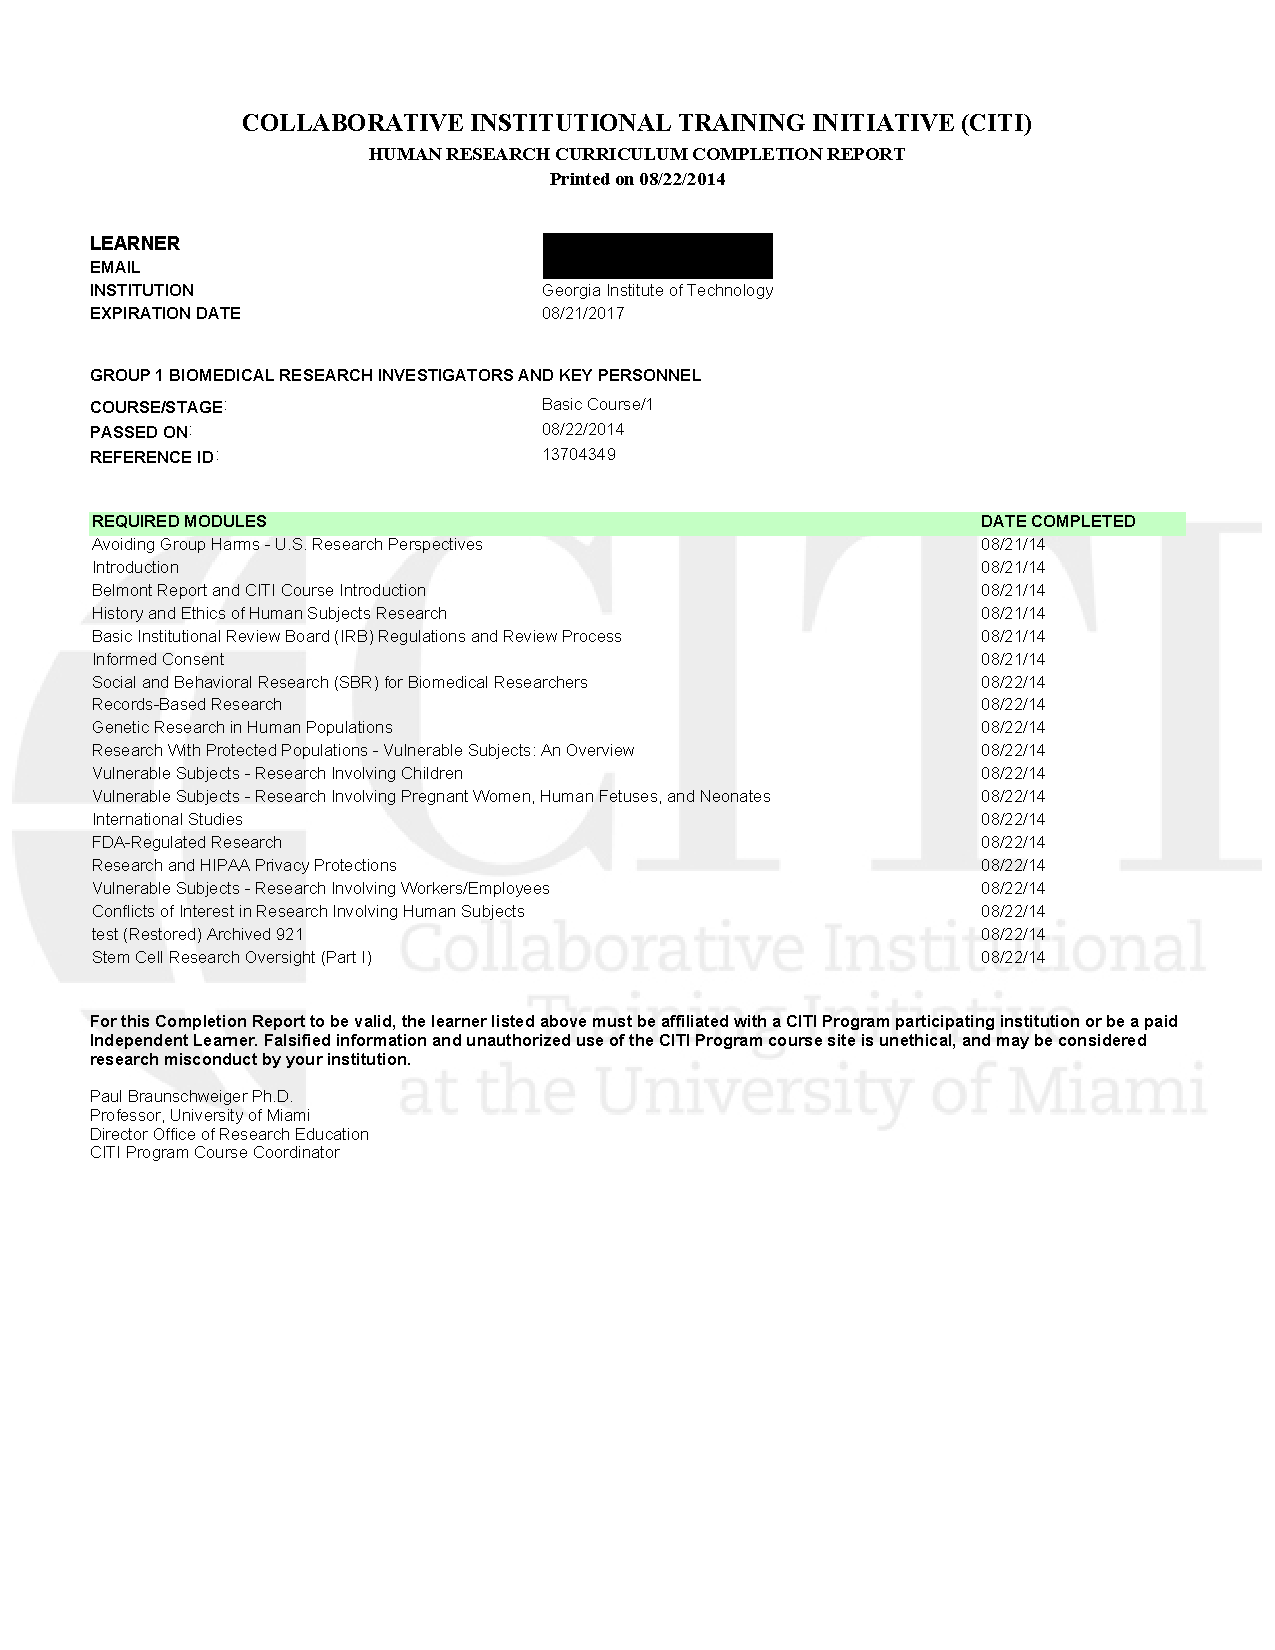
\includegraphics[trim=0 200 0 0,width=\textwidth]{group1.pdf}
\caption{Group 1}
\end{subfigure}
\begin{subfigure}[b]{0.5\textwidth}

\includegraphics[trim=0 200 0 0,width=\textwidth]{group2.pdf}
\caption{Group 2}
\end{subfigure}
\caption{Sample CITI Certification}
\end{figure}
\label{fig:certification}
\end{solution}



\section{Logistic Regression [20 points]}
With a set of historical healthcare data, you could train a Logistic Regression classifier to make prediction. A training set $D$ is composed of $\{(\mathbf{x}_i, y_i)\}_1^N$, where $y_i \in \{0, 1\}$ is the label, and $\mathbf{x}_i\in\mathbf{R}^d$ is the feature vector of the $i$-th patient. In logistic regression we have $p(y = 1 | \mathbf{x}, \mathbf{w}) = \sigma(\mathbf{w}^T\mathbf{x})$, where $\sigma(t) = \frac{1}{1 + \exp{-t}}$ is the sigmod function. 

\textbf{a.} Show the negative \textit{log}-likelihood for $D$, simplify it as much as you can [5 points]

\textbf{b.} Show the gradient of the negative \textit{log}-likelihood in terms of $\mathbf{w}$ [5 points]

\textbf{c.} Show the Hessian of the negative \textit{log}-likelihood [5 points]

\textbf{d.} In order to use gradient descent to find best $\mathbf{w}$, you need to make sure the negative \textit{log}-likelihood is convex. Proof Hessian in question c is positive definite [5 points]

\section{Stochastic Gradient Descent [20 points]}
In previous problem, you studied Logistic Regression learning in batch style. In this problem, you will approach the problem with another method. Suppose your system continuously collects patient data and predicts their severity using \textbf{Logistic Regression}. When patient data vector $\mathbf{x}$ arrive your system, the system need to predict whether he/she is in severe condition(predicted label $\hat{y} \in \{0, 1\}$) and need immediate care or not. The prediction will be delivered to physician and physician will look into the patient. Finally, the physician will provide a feedback(real label $y \in \{0, 1\}$) to your system, so that the system could be updated to make better prediction in the future. In this problem, you are going to derive the equation behind this setting.

\textbf{a.} Show the log likelihood $l$ of a $(\mathbf{x}_t, y_t)$ pair. [5 points]

\textbf{b.} Show how to update the coefficient vector $\mathbf{w}_t$ when you get  patient feature vector $\mathbf{x}_t$ and physician feedback label $y_t$ at time $t$ using $\mathbf{w}_{t-1}$(suppose learning rate $\eta$ is given). ?[5 points]

\textbf{c.} What's the time complexity of the update rule from b if $\mathbf{x}_t$ is very sparse? [2 points]

\textbf{d.} Briefly explain the consequence of too large $\eta$ and too small $\eta$. [3 points]

\textbf{e.} Show how to update $\mathbf{w}_t$ under the penalty of L2 norm regularization. In other words, update $\mathbf{w}_t$ according to $l - \mu \|\mathbf{w}\|^2 $, where $\mu$ is a constant. What's the time complexity? [5 points]

\textbf{f.} When you use L2 norm, you will find each time when you get a new $(\mathbf{x}_t, y_t)$ you need to update every element of vector $\mathbf{w}_t$ even when $\mathbf{x}_t$ only have very few non-zero elements. Show how to update $\mathbf{w}_t$ lazily(hint: update $i$-th element of $\mathbf{w}_{t}$, $\mathbf{w}_{ti}$, only when $i$-th element of $\mathbf{x}_{t}$, $\mathbf{x}_{ti}$, is non-zero, and you have to read this paper \href{http://lingpipe.files.wordpress.com/2008/04/lazysgdregression.pdf}{a paper}). [Extra 5 points]

\newpage
\section{Programming [50 points]}
First, follow the \href{https://sites.google.com/site/classbdh/quick-vm.pdf?attredirects=0}{instructions} to install Cloudera VM if you haven't done that yet. Then you need to download data from AWS S3. We have made the files public, so that you could download them as follows
\begin{lstlisting}[frame=single, language=bash]
wget http://s3.amazonaws.com/cse8803/ICD9EVENT.csv
wget http://s3.amazonaws.com/cse8803/MORTALITYEVENT.csv
wget http://s3.amazonaws.com/cse8803/ICD9_FEATURE_MAP.csv
wget http://s3.amazonaws.com/cse8803/training.data
wget http://s3.amazonaws.com/cse8803/testing.data
\end{lstlisting}

\subsection{Transform data [10 points]}
It's a common practice to convert raw data into some common data format before conducting real machine learning study. If the dimensionality of a feature vector is large but the feature vector is sparse (i.e., only a few nonzero elements), sparse representation should be employed. In this problem you will use ICD9 diagnostic code for each patient to construct the feature vector and represent the feature vector in \href{http://svmlight.joachims.org/}{SVMLight} format. 

You will use diagnostics events of patients. Specifically, each patient is associated with a list of events, and you need to aggregate the same events that satisfy certain criteria into one feature. Some concept you need to know (for details please refer to lectures):
\begin{itemize}
\item Diagnosis date: The day at which event of interest you are to predict. In this homework, you are predicting whether a patient is deceased or not at specific date.
\item Observation Window: The time interval you will use to screen events.
\item Prediction Window: A fixed time interval you will use to make prediction.
\end{itemize}
Suppose a patient was deceased in 2010, while the observation window is 5 years and prediction window is 2 years, you will use diagnostic events between 2004 and 2008 to predict the mortality. 

You will work on following files in \textit{pig} folder
\begin{itemize}
\item \textbf{etl.pig}: Modify this scripts as you need. The sample implementation doesn't consider observation window and prediction window.
\item \textbf{utils.py}: Implement necessary python User Defined Function (UDF) in this file (optional).
\end{itemize}

You will need to use following data files you downloaded from S3:
\begin{itemize}
\item \textbf{MORTALITYEVENT.csv} contains the target label which is one-year after discharge mortality indicator. Each line contains a tuple $(p, label, date)$, 
where $p$ is patient id, label is 0 (alive) or 1 (deceased) and $date$ is the date after 1 year of discharge. 

\item \textbf{ICD9EVENT.csv}: Each line contains a tuple $(p, icd9\_code, date)$, which indicates patient $p$ was diagnosed with $icd9\_code$ at a given $date$. Because a patient can visit the hospital several times and diagnosed with the same ICD9 code, you will need to aggregate $(p, code)$ using COUNT (a pig command).
\item \textbf{ICD9\_FEATURE\_MAP.csv}: You need to map a feature (ICD9 code in this problem)  from its name to an index. This file contains $(index, name)$ pairs for ICD9 codes you will use.
\end{itemize}

Further, in machine learning algorithm like logistic regression, it is important to normalize different feature into the same scale. Modify \textbf{etl.pig} to consider observation window(1000 days) and prediction window(365 days). Then, scale feature values using min-max normalization\href{http://stats.stackexchange.com/questions/70801/how-to-normalize-data-to-0-1-range}{this approach}. Please do not change the input/output location and format. (hint: $min(x_i)$ is zero in this problem)

Run your pig script in local mode, you will need the output for the next question.
\begin{lstlisting}[frame=single,language=bash]
pig -x local etl.pig
\end{lstlisting}
\textbf{Deliverable: pig/etl.pig and pig/utils.py [10 points]}

\subsection{SGD Logistic Regression [20 points]}
In this question, you are going to implement your own Logistic Regression classifier in python using the equations you derived in question \textbf{3.e}. To help you start, a skeleton of code will be provided. Find related files in \textit{lr} folder. You will train and test a classifier by running
\begin{enumerate}
\item cat path/to/training/data \textbar{} python train.py -f 5676
\item cat path/to/testing/data \textbar{} python test.py 
\end{enumerate}
You will use the two sets of training/testing data. One comes from output of previous problem. Another pair of training/testing data set is downloaded from S3 (training.data and testing.data).

To better understand the performance of your classifier, you will need to use standard metrics like AUC. A script file named \textbf{install-conda.sh} is provided to help you install necessary modules for drawing ROC curve. The script is tested in Cloudera VM. You may need to modify it if you want to install that somewhere else. Restart the terminal after installation.

\textbf{a.} Update the \textbf{lrsgd.py} file. You are allowed to add extra methods, but please make sure the existing method names and parameters remain unchanged. Use \href{https://docs.python.org/2/library/}{standard modules} of Python 2.7 only, as we will not guarantee the availability of any third party modules while testing your code. [14 points]

\textbf{b.} Show the ROC curve generated by test.py in this writing report for different learning rates $\eta$ and regulization parameters $\mu$ combination and briefly explain the result. [3 points per dataset]

[Extra 5 points] Implement using result of question \textbf{3.f}, and show the speed up. You could use a larger data set \textit{s3://cse8803/train.large.data}, and the number of features is 299135.

\subsection{Hadoop [20 points]}
In this problem, you are going to train multiple logistic regression classifiers using your implementation of previous problem with Hadoop in parallel. The pseudo code of Mapper and Reducer are listed as Algo~\ref{algo_map} and Algo~\ref{algo_reduce} respectively. Find related files in \textit{lr} folder.

\begin{algorithm}
\SetKwFunction{Random}{Random}\SetKwFunction{Emit}{Emit}
\SetKwInOut{Input}{input}\SetKwInOut{Output}{output}
\Input{Ratio of sampling $r$, number of models $M$, input pair $(k,v)$}
\Output{key-value pairs}
\BlankLine
\For{$i\leftarrow 1$ \KwTo $M$}{
$m\leftarrow$\Random\;
\If{$m < r$}{
\Emit($i,v$)
}
}
\caption{Map function}\label{algo_map}
\end{algorithm}

\begin{algorithm}
\SetKwInOut{Input}{input}\SetKwInOut{Output}{output}
\Input{$(k,v)$}
\Output{Trained model}
Fit model on $v$\;
\caption{Reduce function}\label{algo_reduce}
\end{algorithm}
You need to copy \textit{training.data} into HDFS using command line.
\begin{lstlisting}[language=bash,frame=single]
hdfs dfs -mkdir hw1
hdfs dfs -mkdir hw1/training
hdfs dfs -put training.data hw1/training/
\end{lstlisting}
\textbf{a.} complete the \textbf{mapper.py} according to pseudo code. [6 points]\\
You could train 5 ensembles by invoking
\begin{lstlisting}[language=bash,frame=single]
hadoop jar \
   /usr/lib/hadoop-mapreduce/hadoop-streaming.jar \
  -D mapreduce.job.reduces=5    \
  -files lr \
  -mapper "python lr/mapper.py -n 5 -r 0.4" \
  -reducer "python lr/reducer.py -f 5676" \
  -input hw1/training \
  -output hw1/models
\end{lstlisting}
Notice that you could apply other parameters to reducer. To test the performance of ensembles, copy the trained models to local via
\begin{lstlisting}[language=bash,frame=single]
hdfs dfs -get hw1/models
\end{lstlisting}
\textbf{b.} Complete the \textbf{testensemble.py} to generate the ROC curve. [6 points]
\begin{lstlisting}[language=bash,frame=single]
cat testing.data | python lr/testensemble.py -m models
\end{lstlisting}
\textbf{c.} Compare the performance with that of previous problem. [8 points]

\subsection{Submission}
The folder structure of your submission should be as below. You could display fold structure using \textit{tree} command. All other unrelated files will be discarded during testing.
\begin{lstlisting}[language=bash,frame=single]
<your gtid>-<your gt account>-hw1
|-- homework1answer.pdf
|-- lr
|   |-- lrsgd.py
|   |-- mapper.py
|   |-- testensemble.py
\-- pig
    |-- etl.pig
    \-- utils.py
\end{lstlisting}
Create a tar archive of the folder above with the following command and submit the tar file.
\begin{lstlisting}[language=bash,frame=single]
tar -czvf <your gtid>-<your gt account>-hw1.tar.gz \
  <your gtid>-<your gt account>-hw1
\end{lstlisting}

\end{document}
